\documentclass[border=8pt, multi, tikz]{standalone}
\usepackage{import}
\usepackage{amsmath}
\usepackage{tikz}
\usetikzlibrary{positioning, arrows.meta, calc, shapes, decorations.pathreplacing}

% Define colors
\definecolor{inputcolor}{RGB}{50, 120, 200}
\definecolor{hiddencolor}{RGB}{100, 180, 100}
\definecolor{outputcolor}{RGB}{220, 80, 80}
\definecolor{normcolor}{RGB}{200, 150, 50}
\definecolor{dropoutcolor}{RGB}{150, 150, 150}

\begin{document}

% ============================================================================
% Figure 1: Meta-Learning Network Architecture
% ============================================================================
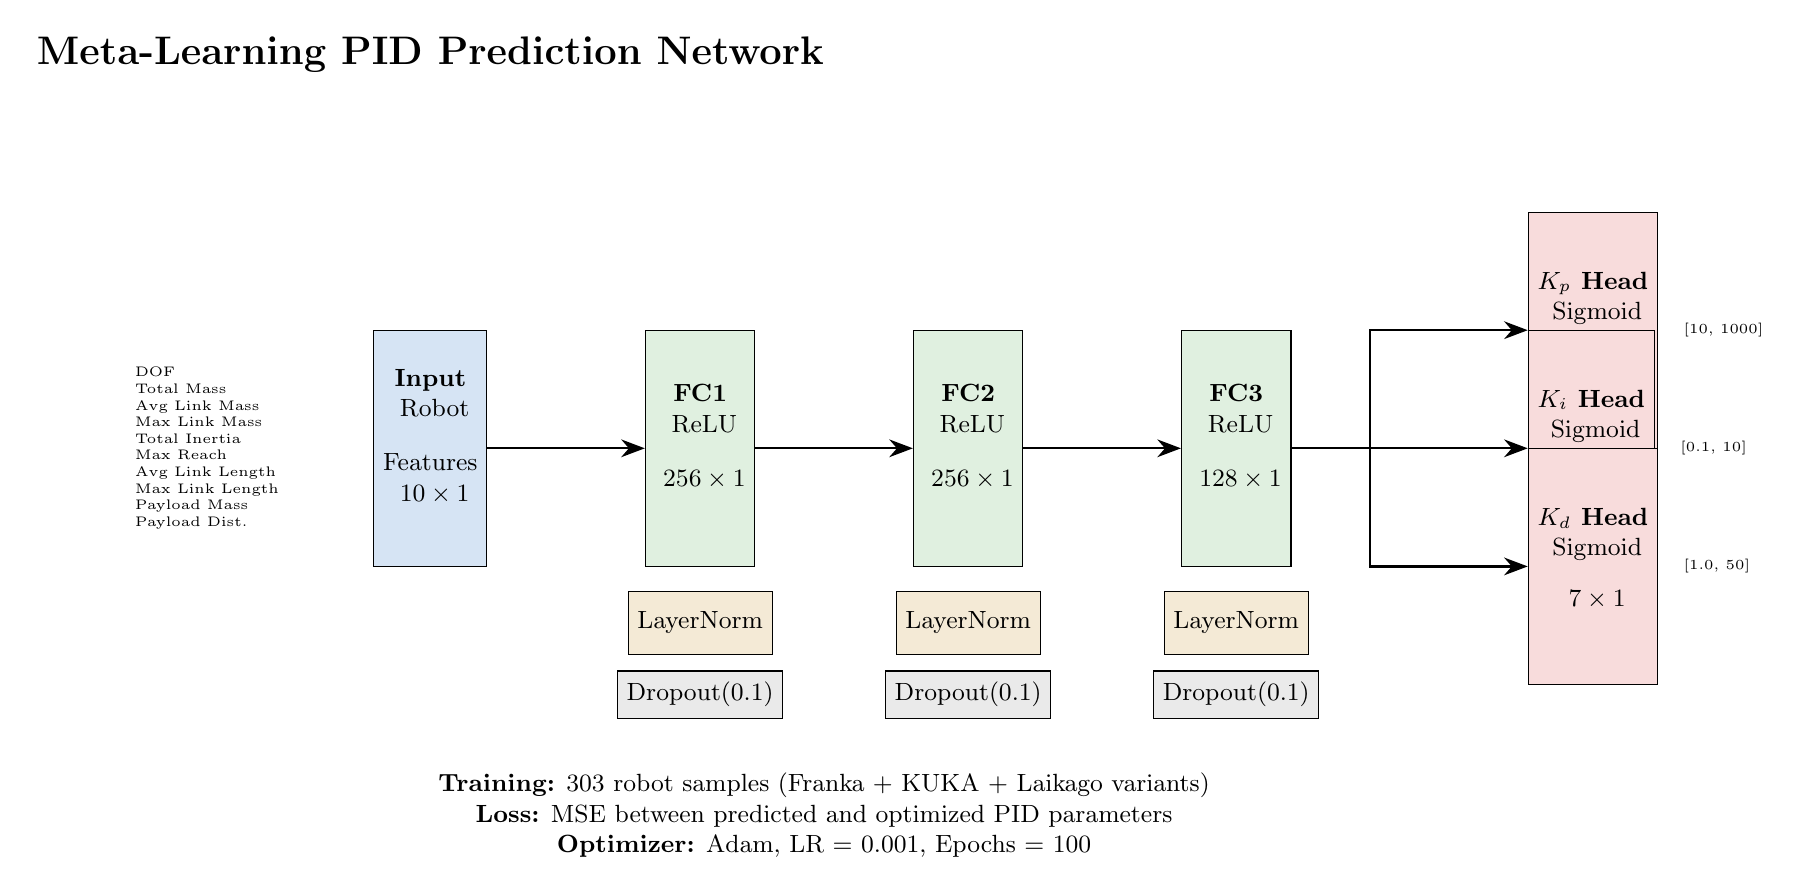
\begin{tikzpicture}[
    node distance=1.5cm and 2cm,
    layer/.style={rectangle, draw, minimum width=1.2cm, minimum height=3cm, align=center, font=\small},
    input/.style={layer, fill=inputcolor!20},
    hidden/.style={layer, fill=hiddencolor!20},
    output/.style={layer, fill=outputcolor!20},
    norm/.style={layer, fill=normcolor!20, minimum height=0.8cm},
    dropout/.style={layer, fill=dropoutcolor!20, minimum height=0.6cm},
    arrow/.style={-{Stealth[length=3mm]}, thick},
    label/.style={font=\footnotesize},
]

% Title
\node[font=\Large\bfseries] at (0, 5) {Meta-Learning PID Prediction Network};

% Input layer
\node[input] (input) at (0, 0) {
    \textbf{Input}\\
    \vspace{0.3cm}
    Robot\\
    Features\\
    \vspace{0.3cm}
    $10 \times 1$
};

% Feature list (left side annotation)
\node[anchor=east, font=\tiny, align=left] at (-1.8, 0) {
    DOF\\
    Total Mass\\
    Avg Link Mass\\
    Max Link Mass\\
    Total Inertia\\
    Max Reach\\
    Avg Link Length\\
    Max Link Length\\
    Payload Mass\\
    Payload Dist.
};

% First hidden layer
\node[hidden, right=of input] (hidden1) {
    \textbf{FC1}\\
    \vspace{0.3cm}
    ReLU\\
    \vspace{0.3cm}
    $256 \times 1$
};

\node[norm, below=0.3cm of hidden1] (norm1) {LayerNorm};
\node[dropout, below=0.2cm of norm1] (dropout1) {Dropout(0.1)};

% Second hidden layer
\node[hidden, right=of hidden1] (hidden2) {
    \textbf{FC2}\\
    \vspace{0.3cm}
    ReLU\\
    \vspace{0.3cm}
    $256 \times 1$
};

\node[norm, below=0.3cm of hidden2] (norm2) {LayerNorm};
\node[dropout, below=0.2cm of norm2] (dropout2) {Dropout(0.1)};

% Third hidden layer
\node[hidden, right=of hidden2] (hidden3) {
    \textbf{FC3}\\
    \vspace{0.3cm}
    ReLU\\
    \vspace{0.3cm}
    $128 \times 1$
};

\node[norm, below=0.3cm of hidden3] (norm3) {LayerNorm};
\node[dropout, below=0.2cm of norm3] (dropout3) {Dropout(0.1)};

% Output heads
\node[output, right=3cm of hidden3, yshift=1.5cm] (kp) {
    \textbf{$K_p$ Head}\\
    \vspace{0.2cm}
    Sigmoid\\
    \vspace{0.2cm}
    $7 \times 1$
};

\node[output, right=3cm of hidden3] (ki) {
    \textbf{$K_i$ Head}\\
    \vspace{0.2cm}
    Sigmoid\\
    \vspace{0.2cm}
    $7 \times 1$
};

\node[output, right=3cm of hidden3, yshift=-1.5cm] (kd) {
    \textbf{$K_d$ Head}\\
    \vspace{0.2cm}
    Sigmoid\\
    \vspace{0.2cm}
    $7 \times 1$
};

% Arrows
\draw[arrow] (input) -- (hidden1);
\draw[arrow] (hidden1) -- (hidden2);
\draw[arrow] (hidden2) -- (hidden3);
\draw[arrow] (hidden3.east) -- ++(1,0) |- (kp.west);
\draw[arrow] (hidden3.east) -- ++(1,0) -- (ki.west);
\draw[arrow] (hidden3.east) -- ++(1,0) |- (kd.west);

% Output range annotations
\node[anchor=west, font=\tiny] at ($(kp.east) + (0.2, 0)$) {[10, 1000]};
\node[anchor=west, font=\tiny] at ($(ki.east) + (0.2, 0)$) {[0.1, 10]};
\node[anchor=west, font=\tiny] at ($(kd.east) + (0.2, 0)$) {[1.0, 50]};

% Bottom annotation
\node[anchor=north, font=\small, align=center] at (5, -4) {
    \textbf{Training:} 303 robot samples (Franka + KUKA + Laikago variants)\\
    \textbf{Loss:} MSE between predicted and optimized PID parameters\\
    \textbf{Optimizer:} Adam, LR = 0.001, Epochs = 100
};

\end{tikzpicture}

\newpage

% ============================================================================
% Figure 2: RL Online Adaptation Network (PPO Actor-Critic)
% ============================================================================
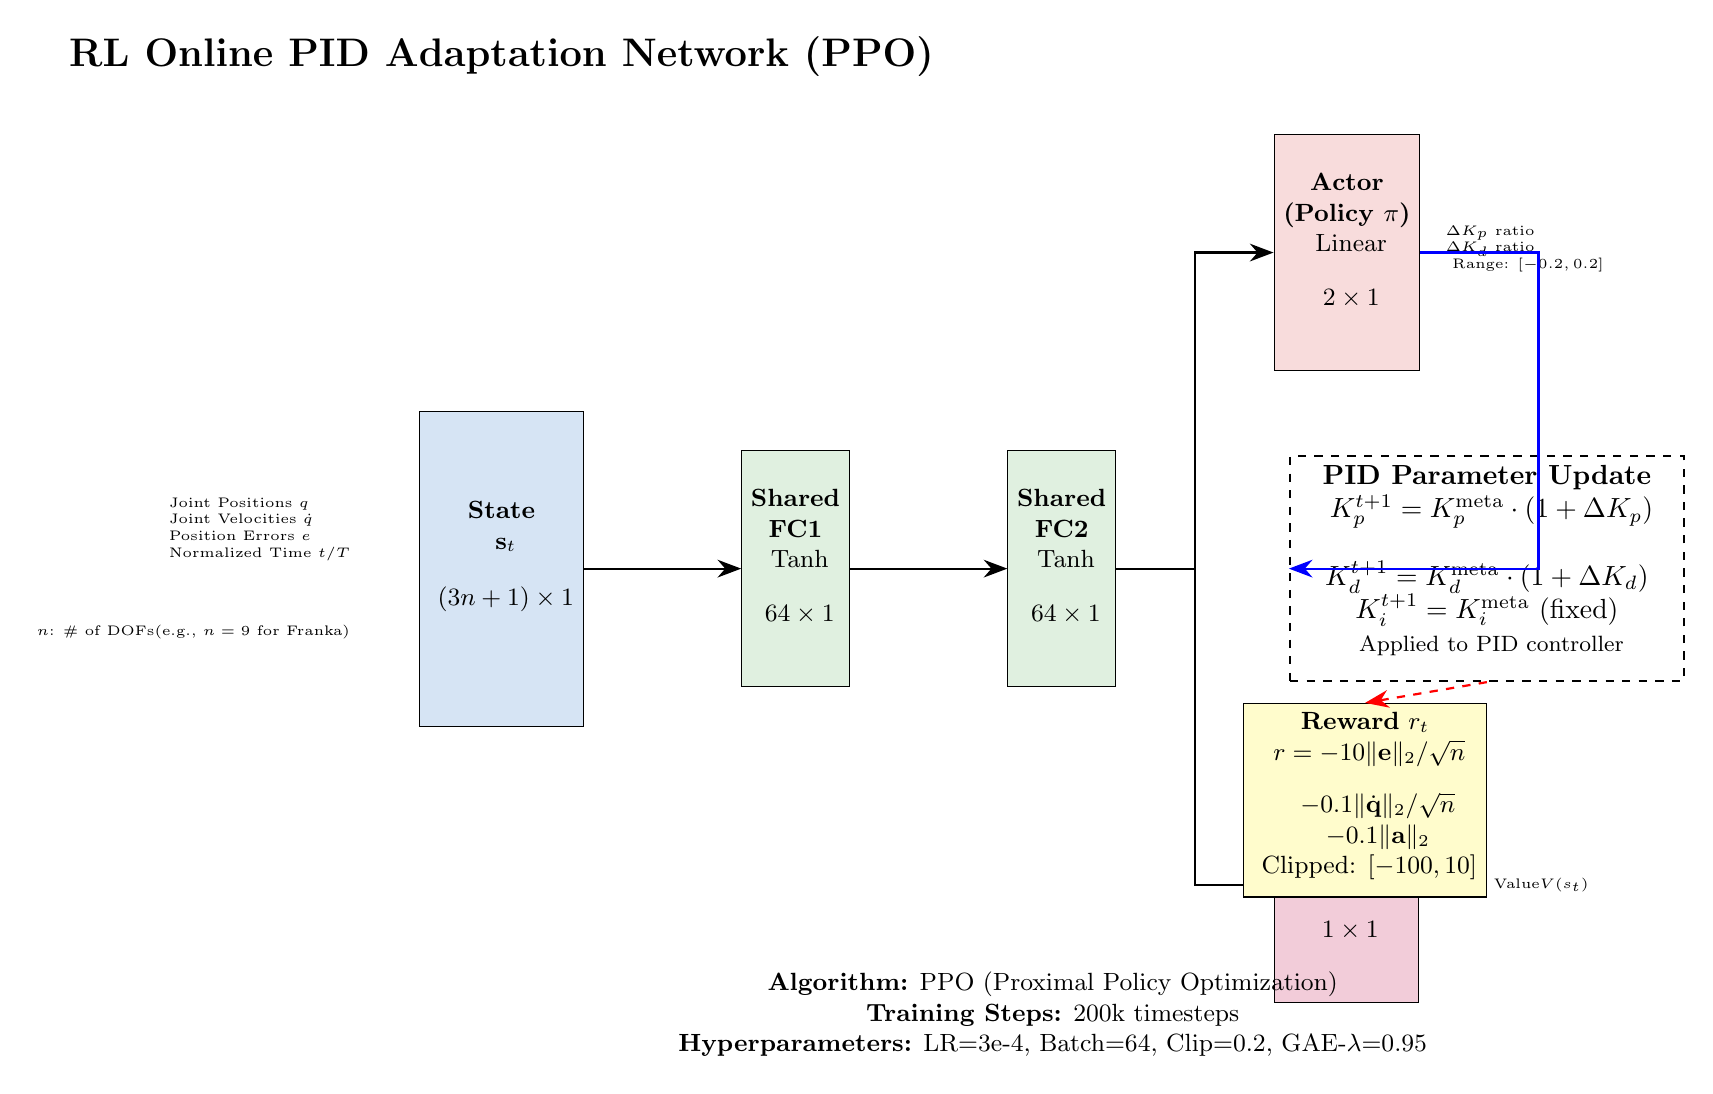
\begin{tikzpicture}[
    node distance=1.5cm and 2cm,
    layer/.style={rectangle, draw, minimum width=1.2cm, minimum height=3cm, align=center, font=\small},
    input/.style={layer, fill=inputcolor!20},
    hidden/.style={layer, fill=hiddencolor!20},
    output/.style={layer, fill=outputcolor!20},
    critic/.style={layer, fill=purple!20},
    arrow/.style={-{Stealth[length=3mm]}, thick},
    label/.style={font=\footnotesize},
]

% Title
\node[font=\Large\bfseries] at (0, 6.5) {RL Online PID Adaptation Network (PPO)};

% Input layer
\node[input, minimum height=4cm] (input) at (0, 0) {
    \textbf{State}\\
    \vspace{0.3cm}
    $\mathbf{s}_t$\\
    \vspace{0.3cm}
    $(3n+1) \times 1$
};

% State components annotation
\node[anchor=east, font=\tiny, align=left] at (-1.8, 0.5) {
    Joint Positions $q$\\
    Joint Velocities $\dot{q}$\\
    Position Errors $e$\\
    Normalized Time $t/T$
};

\node[anchor=east, font=\tiny] at (-1.8, -0.8) {
    $n$: \# of DOFs\\
    (e.g., $n=9$ for Franka)
};

% Shared feature layers
\node[hidden, right=of input] (shared1) {
    \textbf{Shared}\\
    \textbf{FC1}\\
    \vspace{0.3cm}
    Tanh\\
    \vspace{0.3cm}
    $64 \times 1$
};

\node[hidden, right=of shared1] (shared2) {
    \textbf{Shared}\\
    \textbf{FC2}\\
    \vspace{0.3cm}
    Tanh\\
    \vspace{0.3cm}
    $64 \times 1$
};

% Actor branch
\node[output, above right=1cm and 2cm of shared2] (actor) {
    \textbf{Actor}\\
    \textbf{(Policy $\pi$)}\\
    \vspace{0.3cm}
    Linear\\
    \vspace{0.3cm}
    $2 \times 1$
};

\node[anchor=west, font=\tiny, align=left] at ($(actor.east) + (0.2, 0)$) {
    $\Delta K_p$ ratio\\
    $\Delta K_d$ ratio\\
    \vspace{0.1cm}
    Range: $[-0.2, 0.2]$
};

% Critic branch
\node[critic, below right=1cm and 2cm of shared2] (critic) {
    \textbf{Critic}\\
    \textbf{(Value $V$)}\\
    \vspace{0.3cm}
    Linear\\
    \vspace{0.3cm}
    $1 \times 1$
};

\node[anchor=west, font=\tiny] at ($(critic.east) + (0.2, 0)$) {
    State Value\\
    $V(s_t)$
};

% Arrows
\draw[arrow] (input) -- (shared1);
\draw[arrow] (shared1) -- (shared2);
\draw[arrow] (shared2.east) -- ++(1,0) |- (actor.west);
\draw[arrow] (shared2.east) -- ++(1,0) |- (critic.west);

% PID update mechanism
\node[draw, rectangle, thick, dashed, minimum width=5cm, minimum height=2.5cm, 
      anchor=west, align=center] (pid_update) at (10, 0) {
    \textbf{PID Parameter Update}\\
    \vspace{0.3cm}
    $K_p^{t+1} = K_p^{\text{meta}} \cdot (1 + \Delta K_p)$\\
    $K_d^{t+1} = K_d^{\text{meta}} \cdot (1 + \Delta K_d)$\\
    $K_i^{t+1} = K_i^{\text{meta}}$ (fixed)\\
    \vspace{0.2cm}
    \footnotesize{Applied to PID controller}
};

\draw[arrow, blue, thick] (actor.east) -- ++(1.5,0) |- (pid_update.west);

% Reward signal
\node[draw, rectangle, fill=yellow!20, anchor=east, align=center, font=\small] 
     (reward) at ($(pid_update.south) + (0, -1.5)$) {
    \textbf{Reward} $r_t$\\
    \vspace{0.2cm}
    $r = -10 \|\mathbf{e}\|_2 / \sqrt{n}$\\
    $\quad - 0.1 \|\dot{\mathbf{q}}\|_2 / \sqrt{n}$\\
    $\quad - 0.1 \|\mathbf{a}\|_2$\\
    \vspace{0.1cm}
    Clipped: $[-100, 10]$
};

\draw[arrow, red, thick, dashed] (pid_update.south) -- (reward.north);

% Training info
\node[anchor=north, font=\small, align=center] at (7, -5) {
    \textbf{Algorithm:} PPO (Proximal Policy Optimization)\\
    \textbf{Training Steps:} 200k timesteps\\
    \textbf{Hyperparameters:} LR=3e-4, Batch=64, Clip=0.2, GAE-$\lambda$=0.95
};

\end{tikzpicture}

\newpage

% ============================================================================
% Figure 3: Complete System Architecture (Meta-Learning + RL)
% ============================================================================
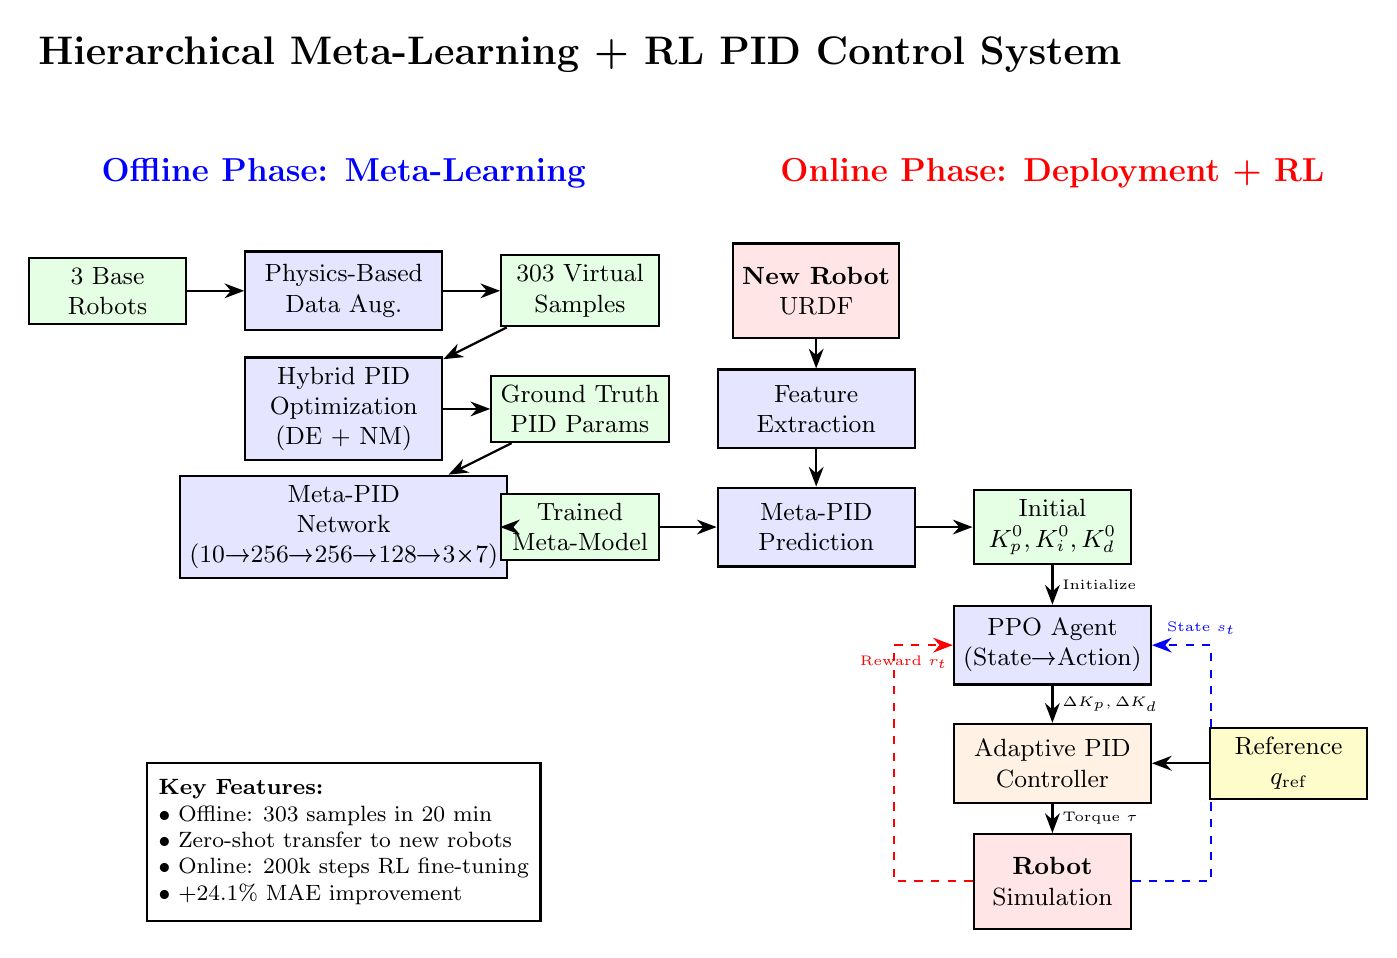
\begin{tikzpicture}[
    node distance=1.2cm and 1.5cm,
    block/.style={rectangle, draw, thick, align=center, font=\small},
    process/.style={block, fill=blue!10, minimum width=2.5cm, minimum height=1cm},
    data/.style={block, fill=green!10, minimum width=2cm, minimum height=0.8cm},
    control/.style={block, fill=orange!10, minimum width=2.5cm, minimum height=1cm},
    robot/.style={block, fill=red!10, minimum width=2cm, minimum height=1.2cm},
    arrow/.style={-{Stealth[length=2.5mm]}, thick},
]

% Title
\node[font=\Large\bfseries] at (6, 8) {Hierarchical Meta-Learning + RL PID Control System};

% ========== OFFLINE PHASE ==========
\node[font=\large\bfseries, blue] at (3, 6.5) {Offline Phase: Meta-Learning};

% Data generation
\node[data] (base_robots) at (0, 5) {3 Base\\Robots};
\node[process] (augmentation) at (3, 5) {Physics-Based\\Data Aug.};
\node[data] (virtual_samples) at (6, 5) {303 Virtual\\Samples};

\draw[arrow] (base_robots) -- (augmentation);
\draw[arrow] (augmentation) -- (virtual_samples);

% Optimization
\node[process] (optimization) at (3, 3.5) {Hybrid PID\\Optimization\\(DE + NM)};
\node[data] (ground_truth) at (6, 3.5) {Ground Truth\\PID Params};

\draw[arrow] (virtual_samples) -- (optimization);
\draw[arrow] (optimization) -- (ground_truth);

% Meta-learning
\node[process] (meta_network) at (3, 2) {Meta-PID\\Network\\(10→256→256→128→3×7)};
\node[data] (meta_model) at (6, 2) {Trained\\Meta-Model};

\draw[arrow] (ground_truth) -- (meta_network);
\draw[arrow] (meta_network) -- (meta_model);

% ========== ONLINE PHASE ==========
\node[font=\large\bfseries, red] at (12, 6.5) {Online Phase: Deployment + RL};

% New robot
\node[robot] (new_robot) at (9, 5) {\textbf{New Robot}\\URDF};
\node[process] (feature_extract) at (9, 3.5) {Feature\\Extraction};
\node[process] (meta_predict) at (9, 2) {Meta-PID\\Prediction};
\node[data] (init_pid) at (12, 2) {Initial\\$K_p^0, K_i^0, K_d^0$};

\draw[arrow] (meta_model.east) -- ++(0.5,0) |- (meta_predict.west);
\draw[arrow] (new_robot) -- (feature_extract);
\draw[arrow] (feature_extract) -- (meta_predict);
\draw[arrow] (meta_predict) -- (init_pid);

% RL adaptation loop
\node[process] (rl_agent) at (12, 0.5) {PPO Agent\\(State→Action)};
\node[control] (pid_controller) at (12, -1) {Adaptive PID\\Controller};
\node[robot] (robot_sim) at (12, -2.5) {\textbf{Robot}\\Simulation};

\draw[arrow] (init_pid) -- node[right, font=\tiny] {Initialize} (rl_agent);
\draw[arrow] (rl_agent) -- node[right, font=\tiny] {$\Delta K_p, \Delta K_d$} (pid_controller);
\draw[arrow] (pid_controller) -- node[right, font=\tiny] {Torque $\tau$} (robot_sim);

% Feedback loop
\draw[arrow, blue, dashed] (robot_sim.east) -- ++(1,0) |- node[above, near end, font=\tiny] {State $s_t$} ($(rl_agent.east) + (0.5, 0)$) -- (rl_agent.east);
\draw[arrow, red, dashed] (robot_sim.west) -- ++(-1,0) |- node[below, near end, font=\tiny] {Reward $r_t$} ($(rl_agent.west) + (-0.5, 0)$) -- (rl_agent.west);

% Reference trajectory
\node[data, fill=yellow!20] (reference) at (15, -1) {Reference\\$q_{\text{ref}}$};
\draw[arrow] (reference) -- (pid_controller);

% Legend
\node[draw, rectangle, thick, minimum width=5cm, minimum height=2cm, align=left, font=\footnotesize]
     at (3, -2) {
    \textbf{Key Features:}\\
    $\bullet$ Offline: 303 samples in 20 min\\
    $\bullet$ Zero-shot transfer to new robots\\
    $\bullet$ Online: 200k steps RL fine-tuning\\
    $\bullet$ +24.1\% MAE improvement
};

\end{tikzpicture}

\end{document}

